\documentclass[twocolumn, 10pt]{article}

% Packages
\usepackage[utf8]{inputenc}
\usepackage{amsmath, amssymb}
\usepackage{graphicx}
\usepackage{geometry}
\usepackage{fancyhdr}
\usepackage{hyperref}
\usepackage{caption}
\usepackage{subcaption}
\usepackage{booktabs}
\usepackage{float}
\usepackage{tikz}
\usepackage{listings}
\usepackage{float}  % For [H] placement
\usetikzlibrary{arrows.meta, positioning}

% Page layout
\geometry{margin=1in}
\pagestyle{fancy}
\fancyhf{}
\rhead{\thepage}
\lhead{Tath Kanchanarin}

% Title
\title{Vehicle Routing Problem with Time Windows}
\author{Tath Kanchanarin}
\date{\today}

\begin{document}

\maketitle


\section*{Problem Statement}
Vehicle Routing Problem with Time Windows (VRPTW) is a well-known
 combinatorial optimization problem, 
 extending the classic Capacitated Vehicle Routing Problem (CVRP).
  It involves determining the optimal set of routes for a fleet
   of vehicles to serve a number of geographically distributed customers,
    each with a specific time interval — known as a time window — during which service must occur with service time at each customer node,
    and each vehicle have limited capacity.

This problem is highly relevant in real-world logistics, where customers and businesses often operate with strict delivery time windows, adding a significant layer of complexity to the standard vehicle routing problem.
There are two common variants of the time window constraint: hard and soft. In the hard time window variant, each customer must be served strictly within the specified interval; violating it renders a solution infeasible. The soft time window variant allows violations at the cost of incurring a penalty cost in the objective function.


The objective of VRPTW is to minimize the total distance traveled by all vehicles while ensuring that each customer is served within their respective time window
 and that vehicle capacity constraints are respected
 . Some other formulations also treat the number of vehicles, minimizing cost for vehicle usage, and waiting time, incurring cost when waiting on nodes as a secondary objective but in this project, we assume an unlimited fleet size that does not require setup costs is provided and waiting time is permitted implicitly with no penalty cost.
 Thus, the only optimization criterion is the total Euclidean (L2) travel distance across all routes with only constraints of time window and capacity of each vehicle.
\begin{figure}[htbp]
    \centering
    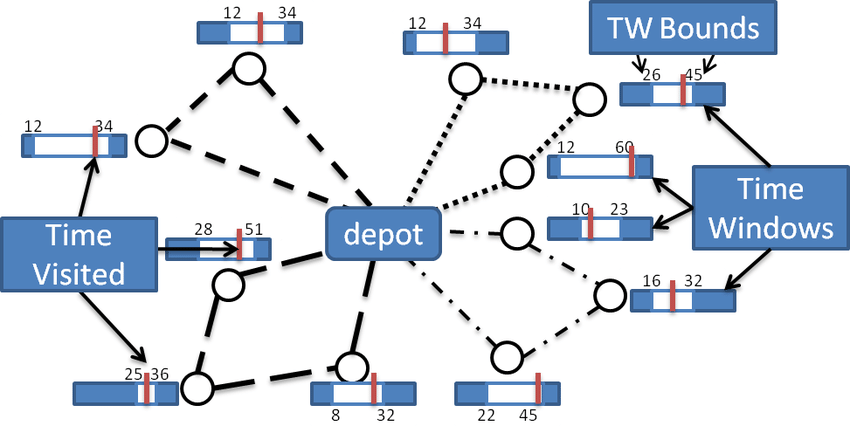
\includegraphics[width=\linewidth]{figures/figures.png}
    \caption{ VRPTW instance with depot and customer time windows \cite{fig_cvrptw}}
    \label{fig:problem_statement}
\end{figure}


Mathemathically, VRPTW is defined on a directed graph \(G = (V, A)\), where \(V\) is the set of nodes and \(A\) is the set of arcs (we will use Distance Matrix instead but they are equivalent). The depot is represented by two nodes: \(0\) (start) and \(n+1\) (return), while the rest are customers.

Each nodes \(i \in V\) has an associated time window \([a_i, b_i]\), where:
\begin{itemize}
    \item \(a_i\) is the earliest time at which service can start,
    \item \(b_i\) is the latest time by which service must be completed,
    \item \(s_i\) is the service duration at node \(i\).
    \item \(t_{ij}\) is the travel time between nodes \(i\) and \(j\).
\end{itemize}

For simplicity, we assume that depot at node 0 and n+1 have \([a_0, b_0]\) = \([a_n+1, b_n+1]\), where they are the earlist and latest time service can start at depot,
with \(s_0\) = \(s_{n+1}\) =  \(q_{0}\) =  \(q_{n+1}\) = 0; servicing time. and load constraint is 0.

\subsubsection*{feasibility condition}
A commonly used feasibility condition on the depot's time window is:
\[
b_0 \geq \max_{i \in V \setminus \{0\}} \left\{ \max\left\{ a_0 + t_{0i},\ a_i \right\} + s_i + t_{i, n+1} \right\}
\]
This bit of constraint ensures the following:
\begin{itemize}
    \item $a_0 + t_{0i}$: Earliest possible arrival at customer i, assuming you depart from the depot as early as possible.
    \item $a_i$: Earliest time you’re allowed to serve customer i.
    \item $\max\{a_0 + t_{0i}, a_i\}$: Actual service start time at i, respecting both the travel time and time window.
    \item $s_i$: service duration at customer i.
    \item $t_{i,n+1}$: travel time to return from customer i to the end depot.
\end{itemize}

This condition checks wheter or not each of the customers can be served within the time window individually, if any of the trip from any
customers is more than b0, then there will not be solution that 
depot cannot serve all customer within the time window.
Since solomon is already have a valid solution, we will ignore this preprocessing step.


\section*{Methodology and Implementation}
\subsection*{IP formulation}

The model that we will be using follows VRPTW1 \cite{toth_vigo_vrp} 
\subsubsection*{Sets and Indices}
\begin{itemize}
    \item $V$ – Set of all nodes, including the depot ($0$) and end depot ($n+1$)
    \item $N$ – Set of customer nodes, i.e., $V \setminus \{0, n+1\}$
    \item $A$ – Set of directed arcs between nodes
    \item $K$ – Set of vehicles
    \item $\delta^+(i)$ – Set of nodes reachable directly from node $i$
    \item $\delta^-(i)$ – Set of nodes that can reach node $i$
\end{itemize}

\subsubsection*{Parameters}
\begin{itemize}
    \item $c_{ij}$ – Distance or cost of traveling from node $i$ to $j$
    \item $t_{ij}$ – Travel time from $i$ to $j$
    \item $[a_i, b_i]$ – Time window for service at node $i$
    \item $s_i$ – Service duration at node $i$
    \item $q_i$ – Demand of customer $i$
    \item $Q$ – Capacity of each vehicle
\end{itemize}

\subsubsection*{Decision Variables}
\begin{itemize}
    \item $x_{ijk} \in \{0, 1\}$ – 1 if vehicle $k$ travels from node $i$ to $j$, 0 otherwise
    \item $T_{ik} \in \mathbb{R}_+$ – Time at which vehicle $k$ starts service at node $i$
\end{itemize}


Decision Variable
\begin{align*}
    x_{ijk} &= \begin{cases}
        1 & \text{if vehicle k travels from customer i to j} \\
        0 & \text{otherwise}
    \end{cases} \\
    T_{ik} &= \text{arrival time of customer i for vehicle k} \\
    q_k &= \text{current load of vehicle k}
\end{align*}


\begin{align}
    \quad \min \sum_{k \in K} \sum_{(i,j) \in A} c_{ij} x_{ijk} && \tag{5.1} \\
    \sum_{k \in K} \sum_{j \in \delta^+(i)} x_{ijk} &= 1 && \forall i \in N \tag{5.2} \\
    \sum_{j \in \delta^+(0)} x_{0jk} &= 1 && \forall k \in K \tag{5.3} \\
    \sum_{i \in \delta^-(j)} x_{ijk} - \sum_{i \in \delta^+(j)} x_{jik} &= 0 && \forall k \in K,\, \forall j \in N \tag{5.4} \\
    \sum_{i \in \delta^-(n+1)} x_{i,n+1,k} &= 1 && \forall k \in K \tag{5.5} \\
    x_{ijk} \cdot (T_{ik} + s_i + t_{ij} - T_{jk}) &\leq 0 && \forall k \in K,\, (i, j) \in A \tag{5.6} \\
    a_i \leq T_{ik} &\leq b_i && \forall k \in K,\, i \in V \tag{5.7} \\
    \sum_{i \in N} q_i \sum_{j \in \delta^+(i)} x_{ijk} &\leq Q && \forall k \in K \tag{5.8} \\
    x_{ijk} &\in \{0, 1\} && \forall k \in K,\ (i, j) \in A \tag{5.9}
\end{align}

\begin{description}
    \item[5.1] Objective function: Minimizes the total travel distance. Here, $c_{ij}$ is the distance between customers $i$ and $j$, and $x_{ijk}$ is a binary decision variable indicating whether vehicle $k$ travels from $i$ to $j$.
    
    \item[5.2] Each customer is visited exactly once by one vehicle.

    \item[5.3] Each vehicle leaves the depot exactly once. (This may be relaxed later.)

    \item[5.4] Flow conservation: Ensures that the number of vehicles entering each customer node equals the number leaving it.

    \item[5.5] Each vehicle must return to the depot (duplicated as node $n+1$).

    \item[5.6] Time consistency: Ensures that the arrival time at customer $j$ is after the departure from $i$, accounting for service and travel time.

    \item[5.7] Time windows: Enforces that customer $i$ is visited within its time window $[a_i, b_i]$.

    \item[5.8] Capacity constraint: Ensures that the total demand served by each vehicle does not exceed capacity $Q$.

    \item[5.9] Binary constraint: Each decision variable $x_{ijk}$ is binary.
\end{description}

constraint 5.3, 5.4, 5.5 ensures subtour elimination and valid solution by ensuring that each vehichle start and at the depot, 
which is different from another formulation that uses Miller-Tucker-Zemlin (MTZ) constraints to eliminate subtours.
This formulation is computationally worse than MTZ, but it is easier to implement and understand.

constraint 5.6 can be split into two
subcases
\begin{itemize}
    \item $x_{ijk} = 1$, then $T_{jk} \geq T_{ik} + s_i + t_{ij}$, making sure arrival at the next customeris after the service time and travel time from previous customer
    \item $x_{ijk} = 0$, then $0\leq 0$ which is trivial
\end{itemize}
constraint 5.7 needs to be applied with indicator variable, since if $x_{ijk} = 0$, then $T_{ik}$ can be any irrevant dummy varialbe, but if $x_{ijk} = 1$, then $T_{ik}$ must be within the time window.


our implementation follows the above formulation closely in python, supplemented with .ipynb file alongside the report. 




\section*{Experiment}
The experiment is conducted on a set of standard benchmark instances from the Solomon's dataset \cite{solomon_dataset}, which
is consited of 25/50/100 customer nodes, with specific flag of clustered(C), randomly(R), randomly clustered(RC) indicating the type of customer distribution on the plane.
The experiment is conducted on macbook pro with m3 max chip and 32GB of RAM, under python 3.10.18 environment with CPLEX version: 22.1.1.0, licensed for academic use through 
python API docplex wrapped jupyter notebook with no thread limits and timeout limtations on solver.

The dataset is expected to be output in the format of "$|X|, |T|, |X|+ |T|, elapsed\_time, Z$", where X is 
the number of edges representing route from customer to customer under a bus, T is the time window constraint of each customer, and Z is the objective value of the solution. 
Then is aggregated under pandas dataframe to be displayed in the report with matplotlib.

The experiment is conditioned on two variants, no limit on number of vehicles being routed by adjusting the constraint 5.3 and 5.5, number of vehicles out and in from depot to be at most 1, 
and the second variant is where we cheat by setting the number of vehicle to be the number of the optimal solution to gain insights and reduce run time by cutting searching space. 
\section*{Results}
Firstly, the computation time for the first variant, where no limit on number of vehicle is set, breaks CPLEX at 25 customers node specifically at C102 and beyond, 
thus the second variant will be the focal point of the experiment.

\subsubsection*{25 Customer Solution Quality}
CPLEX is able to solve almost all of the instances of 25 customers, with the exceptoin of R110 and R111, where R110 is the instance with no solution, but R111 was terminated by hand. 
Below is the table of comparisoin between the known optimal solution and CPLEX solution.
\begin{table}[H]
\centering
\caption{Percentage gap between CPLEX results and benchmark optimal solutions for Solomon 25 customer}
\label{tab:percentage_gap}
\begin{tabular}{lr}
\toprule
Instance & Percentage Gap \\
\midrule
C101 & 0.268489 \\
C102 & 0.229968 \\
C103 & 0.229968 \\
C104 & 0.293984 \\
C105 & 0.268489 \\
C106 & 0.268489 \\
C107 & 0.268489 \\
C108 & 0.268489 \\
C109 & 0.268489 \\
C201 & 0.392438 \\
C202 & 0.392438 \\
C203 & 0.392438 \\
C204 & 0.389521 \\
C205 & 0.392438 \\
C206 & 0.392438 \\
C207 & 0.389761 \\
C208 & 0.407234 \\
R101 & 0.199306 \\
R102 & 0.184211 \\
R103 & 0.241584 \\
R104 & 0.254552 \\
R105 & 0.195785 \\
R106 & 0.232104 \\
R107 & 0.228264 \\
R108 & 0.250367 \\
R109 & 0.300295 \\
R111 & 12.063059 \\
R112 & 0.532028 \\
R201 & 0.231965 \\
R202 & 0.240534 \\
R203 & 0.236379 \\
R204 & 0.251148 \\
R205 & 0.270233 \\
R206 & 0.289378 \\
R207 & 0.286116 \\
R208 & 0.345369 \\
R209 & 0.232497 \\
R210 & 0.217092 \\
R211 & 0.288048 \\
RC101 & 0.229006 \\
RC102 & 0.268411 \\
RC103 & 0.336129 \\
RC104 & 0.175800 \\
RC105 & 0.261752 \\
RC106 & 0.291012 \\
RC107 & 0.217848 \\
RC108 & 0.167891 \\
RC201 & 0.289013 \\
RC202 & 0.243755 \\
RC203 & 0.242658 \\
RC204 & 0.178364 \\
RC205 & 0.274971 \\
RC206 & 0.340873 \\
RC207 & 0.217848 \\
RC208 & 0.288669 \\
\bottomrule
\end{tabular}
\end{table}
The percentage gap have mean of 1.5906213476904933\% and standard deviation of 0.4928704901050774\%, without R111,
the mean and std becomes 0.07213788788994965\%, 0.2786077471971899\%. The formulation is very effective in terms of accuracy.

\subsubsection*{25 Customer Solution runtime}
Based on 25 customers data set generally Clustered dataset has the best perfomance, with shortest runtime followed by random clustered dataset, and random dataset having the longest runtime.
\begin{figure}[H]
    \centering
    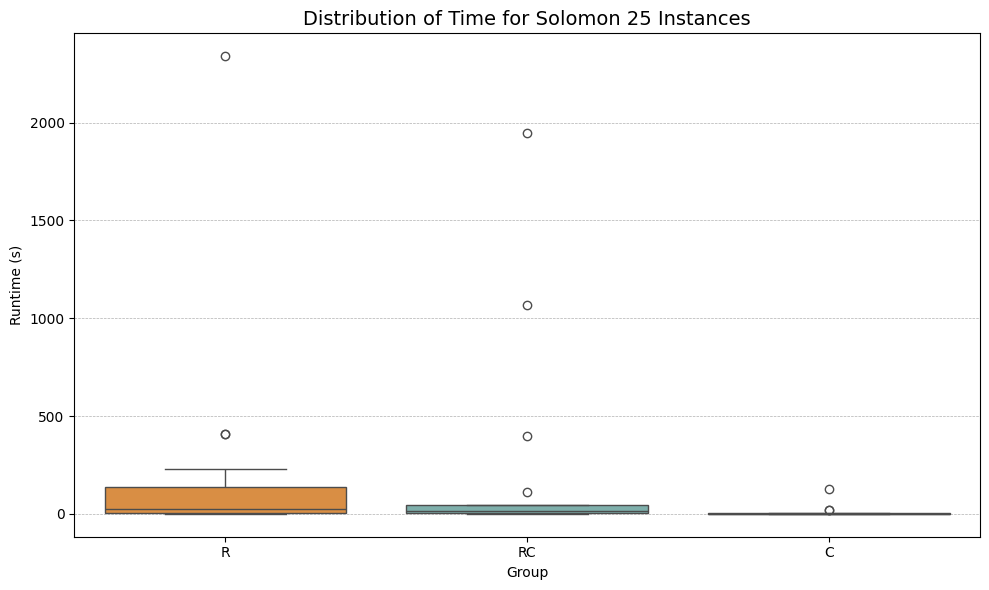
\includegraphics[width=\linewidth]{figures/25_dist.png}
    \caption{distribution of runtime for 25 customers in seconds}
    \label{fig:variable_growth}
\end{figure}

\subsubsection*{50 and 100 Customers}
current formulation is not able to solve most 50 and 100 customers dataset,
breaking in most cases except for C101 for 50 and 100 customers, and C102 for 50 customers.
With so many little data points, it is hard to draw any conclusion on both solution quality and runtime. 



\subsubsection*{Variable and Constraint Growth}
\begin{figure}[H]
    \centering
    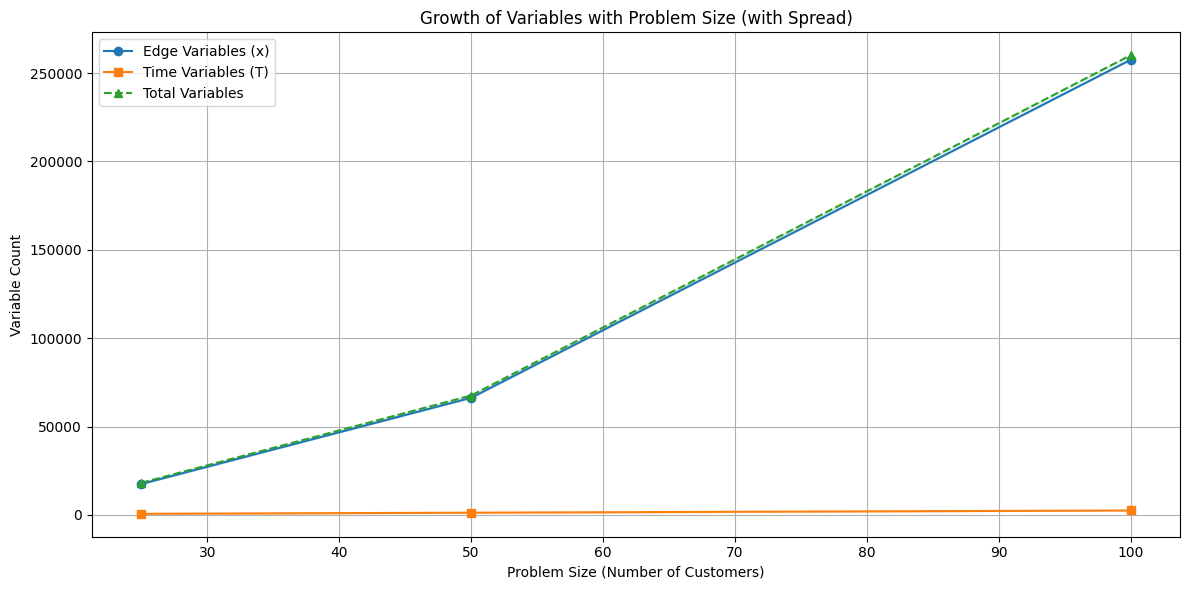
\includegraphics[width=\linewidth]{figures/variable_count.png}
    \caption{Average number of variables for each dataset, at 25, 50 and 100 customers   }
    \label{fig:varialbe_count}
\end{figure}
\begin{figure}[H]
    \centering
    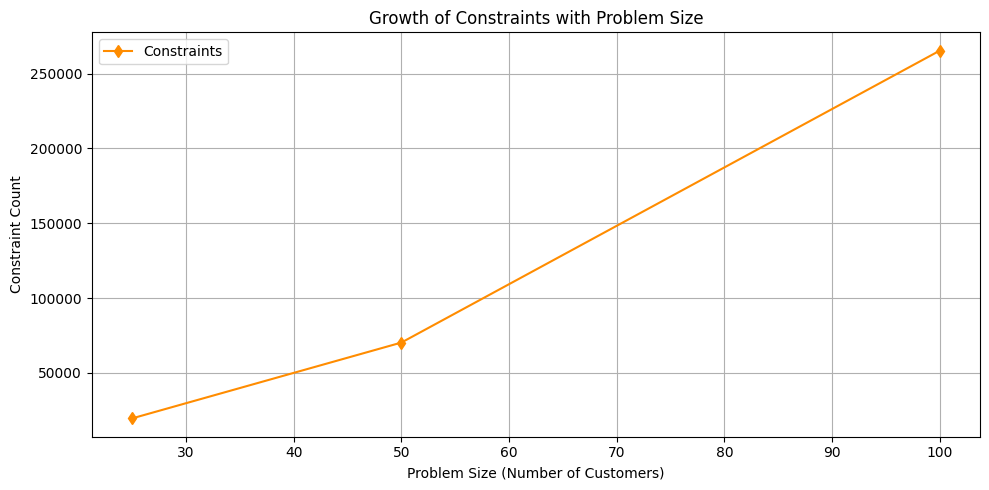
\includegraphics[width=\linewidth]{figures/constraint_size.png}
    \caption{Average number of constraint for each dataset, at 25, 50 and 100 customers  }
    \label{fig:constraint_size}
\end{figure}

The dataset somewhat show explosive growth of the variables and constraints as it is shown to jump from 10k to 100k decision variables within 100 customers

For dataset of 50 customers, the runtime is sub one second for the first cluster set, then for the rest the program freezes
and Cplex does not terminate.
For dataset of 100 customers, CPLEX crashed and burned due to running out of memory, so experiments beoyond 50
customers calls for better algorithm/ formulation to solve the problem.



\section*{Analysis and Discussion}
As shown in the results section, the accuracy of the model is very high except for one instance, it is my opinion that 
this is due to numerical rounding instead of the model itself, as 0.3\% is very small percentage gap to be considered another solution.
Ideally the solution could be validated, but the optimal solution is not available for us.
Aside from that, it is clear that
Vehicle Routing Problem with Time Windows (VRPTW) is computationally challenging, 
especially as problem size increases.
A key issue is the rapid growth of decision variables—particularly
the binary arc variables \( x_{ijk} \)—which scale cubically with the number of customer nodes and number of vehicles.
Specifically, the number of edges is \( O(|V|^2) \), and with each vehicle \( k \), 
the number of variables grows to \( O(|V|^2 \cdot |K|) \). 
Although the number of vehicles \( |K| \) is 
typically fixed (e.g., around 10 in the Solomon dataset), this growth, reflected in the figures above, still leads to an explosive number of variables.
and 
since each variable is binary integer. variable, they are subjected to branch-and-bound search, which further increases computational expense. 

The runtime result for 25 customers show 
runtime varies significantly by dataset structure with the clustered dataset achieving the shortest runtimes, random clustered datasets following, and purely random datasets exhibiting the longest runtimes.

This is to be expected, since clustered dataset has more limited search space, and thus less spaces to perform branch and bound on, while random dataset has the more space to branch and bound on, thus the longest runtime.
It is to be noted however that the distribution of runtime is very random due to mulitple factors,
random input, CPLEX's internal heuristics, so this distribution is not the representation of the actual runtime, 
but rather a representation of the runtime of the solver on the specific dataset. 
Generally the trend from experiment is 
that the runtime is either sub one second, or 2000 seconds, or does not terminate at all, the extreme cases
make it hard to draw any conclusion on the runtime perfomance of the solver. 
The fact that distance can plays a role in runtime in unknown ways make it harder to draw any conclusion of what causes 
CPLEX to break. Distance plays a a role but its effect remains unclear.

Overall, the results suggest that exact methods such as branch-and-bound
 are not practical for solving large VRPTW instances.
  Even a state-of-the-art solver like CPLEX struggles under default configurations. 
  This underlines the need for more scalable solution techniques, 
  such as heuristics and metaheuristics—e.g., genetic algorithms, simulated annealing, 
  or ant colony optimization—which are better suited to navigating the vast combinatorial search space of VRPTW in reasonable time at the 
  cost of optimality.


\section*{Conclusion}

This report presented a mathematical formulation and computational study
 of the Vehicle Routing Problem with Time Windows (VRPTW) 
 using a mixed-integer programming (MIP) approach.
  The formulation captures both capacity and time window constraints, 
  with the primary objective of minimizing total Euclidean travel distance. 
  Assumptions included an unlimited fleet size, no penalty for waiting time, and valid preprocessing conditions.

Computational experiments 
conducted on Solomon benchmark datasets revealed that the model is capable of 
producing near-optimal solutions for instances with up to 25 customers.
 However, as the instance size increases,
  the model exhibits exponential growth in the number of binary decision variables—scaling as \(O(|V|^2 \cdot |K|)\)—and 
  consequently suffers from significant performance degradation in terms of both runtime and memory usage.
   In particular, CPLEX was unable to solve several instances beyond 25 customers under default configurations.

The analysis further indicates that problem structure significantly 
affects solver performance:
 clustered customer distributions lead to
  substantially faster convergence than random or mixed distributions, 
  due to a more constrained and localized feasible region.

In summary, while the MIP formulation provides a
 rigorous framework for modeling VRPTW
 , its scalability and time-feasibility is limited. These findings highlights the need for alternative 
 solution techniques such as better decomposition methods and heuristics to tackle larger instances effectively.


\bibliographystyle{plain}

\bibliography{refs}
% Uncomment below if using BibTeX
% \bibliography{yourbibfile}

\end{document}